\documentclass[11pt]{article}
\usepackage{titlesec}

\usepackage{titlesec}

\titleformat{\section}
  {\centering\Large\bfseries} % Style: centered, large font, bold
  {}                          % No section number
  {0em}                       % Spacing between number and title
  {}                          % Title content (unchanged)

\titleformat{\subsection}
  {\normalfont\Large\bfseries}   % Formatting style: font, size, bold, etc.
  {}                             % Empty to suppress numbering
  {0em}                          % Spacing between label and title (ignored here)
  {}                             % Code before the title

\renewcommand{\abstractname}{\Large Abstract} % Change title size (if required)
\renewenvironment{abstract}
  {\begin{center}\bfseries\Large Abstract\vspace{1em}\end{center}%
   \normalsize} % Adjust text size here
  {}

\usepackage{amsmath, amssymb}
\usepackage{xcolor}
\usepackage{enumerate}
\usepackage{graphicx}
\usepackage{tabularx}
\usepackage{algorithm}

\usepackage{algpseudocode}
\usepackage{tikz}
\usepackage{tikz-qtree}
\usepackage{subcaption}

\usepackage{natbib}  % For bibliography
\usepackage{hyperref}  % For clickable links

\usepackage{indentfirst}

%
% Basic Document Settings
%  

\topmargin=-0.45in
\evensidemargin=0in
\oddsidemargin=0in
\textwidth=6.5in
\textheight=9.0in
\headsep=0.25in

\linespread{1.1}

\usepackage{listings}
\lstset{
  language=Python,                   % Set programming language
  keywordstyle=\bfseries\color{blue},% Bold keywords in blue
  stringstyle=\color{teal},          % Strings in teal
  commentstyle=\itshape\color{red}, % Italicize comments in gray
  frame=lines,                       % Add lines at the top and bottom
  rulecolor=\color{gray!30},         % Light gray for the frame
  tabsize=4,                         % Set tab size to 4 spaces
  captionpos=b,                      % Place caption below the code
  emphstyle=\bfseries\color{purple}, % Highlight emphasized text
  escapeinside={(*@}{@*)},           % Allows for LaTeX inside code
  extendedchars=true                 % Support extended characters
}



% headers, footers, titles
\newcommand{\CourseName}{SI140A Probability and Statistics Final Project}
\newcommand{\DueDate}{2025/1/12 10:59pm}


\title{
    \vspace{100pt}
    \bigskip
    \textbf{\CourseName:} \\
    \textbf{Performance Evaluation of Bandit Learning Algorithms} \\
    \bigskip
}
\author{Jingran Fan \and Anrui Wang \and Zhao Lu}
\bigskip
\date{Due date: \DueDate}

\begin{document}
\setlength{\parindent}{2em}

\maketitle

\newpage

\begin{abstract}

Multi-armed bandit problems are fundamental models in sequential decision-making under uncertainty, wherein an agent must choose from several options (arms) over repeated trials to maximize cumulative rewards. These problems capture the delicate balance between exploration—seeking information about less-known options—and exploitation—leveraging current knowledge to select the best option. Classical bandit learning algorithms, such as 
$\epsilon$-greedy, Upper Confidence Bound (UCB), and Thompson Sampling (TS), have been extensively studied and form the cornerstone of modern reinforcement learning techniques. More recently, Bayesian approaches that incorporate prior beliefs and update them with observed data have gained traction, offering theoretical elegance and robust performance in a variety of settings.

This project focuses on evaluating the performance of well-known bandit algorithms through numerical experiments. In Part I, we consider classical bandit algorithms operating on Bernoulli arms with parameters provided by an oracle. Although the oracle’s parameters and optimal attainable reward (the “oracle value”) are unknown to the algorithms, they provide a ground truth reference for performance comparison. We implement and benchmark 
$\epsilon$-greedy (with various $\epsilon$-values), UCB (with different confidence scales), and TS (with varying Beta priors) under identical experimental conditions. By analyzing their regret—defined as the gap between the algorithm’s cumulative reward and the oracle value—we investigate how tuning parameters and prior knowledge impacts the exploration-exploitation trade-off.

In the optional Part II, we extend our analysis to a Bayesian bandit setting with discounted rewards, where prior distributions on arm parameters are continuously updated as more data is observed. We examine intuitive heuristics and discuss why these heuristics may fail to achieve optimality. Furthermore, we explore the derivation of optimal policies through recursive equations and investigate practical methods for exact and approximate solutions.

Overall, this project aims to provide a rigorous empirical evaluation of both classical and Bayesian bandit algorithms. By comparing their performance and understanding their underlying trade-offs, we gain deeper insights into bandit learning theory and develop intuition for selecting and designing effective strategies in diverse applications.
\end{abstract}

\newpage

\tableofcontents

\newpage

\newpage
\section{Introduction}

In many real-world scenarios—from online advertising to medical trials—decision-makers must choose actions to maximize cumulative rewards. However, these decisions also provide valuable information that can guide future actions. This creates a fundamental tension between exploiting what we already know to gain immediate benefits and exploring new options to potentially improve future outcomes. This challenge is central to the field of reinforcement learning and is known as the exploration-exploitation trade-off.

A classic illustration is the multi-armed bandit problem. Imagine walking into a casino and facing a slot machine with multiple arms, each offering a different, unknown payoff distribution. Your goal is to pull the arms over a sequence of trials to earn as many rewards as possible. Since you do not know which arm is best, you must try them out (exploration) while continuing to play the arm that seems most promising (exploitation). Crucially, the reward probabilities remain fixed but hidden, and the only way to learn them is by experimenting.

This report examines three classical strategies for solving the multi-armed bandit problem—
$\epsilon$-greedy, Upper Confidence Bound (UCB), and Thompson Sampling (TS). By comparing their performance, we gain insight into how they balance exploration and exploitation and how well they adapt to uncertain, reward-driven environments.

\newpage
\section{Part I: Classical Bandit Algorithms}
\subsection{Problem 1}
Choose $N = 5000$ and compute the theoretically maximized expectation of aggregate rewards over $N$ time slots. Suppose we have an oracle that provides the parameters of the Bernoulli distributions for three arms as follows:
\[
\theta_1 = 0.7, \quad \theta_2 = 0.5, \quad \theta_3 = 0.4.
\]

We choose the time horizon as \( N = 5000 \) time steps. If we know these parameters beforehand (as the oracle does), the strategy to maximize the expected total reward is to always pull the arm with the highest success probability, which in this case is arm 1 (with \(\theta_1 = 0.7\)).

The expected reward is:
\[
\max_{I(t), t = 1, \dots, N} \mathbb{E} \left[ \sum_{t=1}^{N} r_{I(t)} \right] = N \times \theta_1 = 5000 \times 0.7 = 3500.
\]

Thus, the theoretically maximized expectation is: $\boxed{3500.}$

\newpage
\subsection{Problem 2}

\subsubsection*{Imports and parameters:}
\lstinputlisting{code/2_0.py}

\subsubsection*{Implementation of $\epsilon$-greedy algorithm:}
\lstinputlisting{code/2_1.py}

\subsubsection*{Implementation of UCB algorithm:}
\lstinputlisting{code/2_2.py}

\subsubsection*{Implementation of Thompson Sampling algorithm:}
\lstinputlisting{code/2_3.py}

\newpage
\subsection{Problem 3}
The results for the three algorithms with various parameters, averaged over 200 trials and 5000 time slots, are presented below:

\subsubsection*{\(\varepsilon\)-Greedy}
\begin{itemize}
    \item \(\varepsilon = 0.1\): \textbf{3408.44}
    \item \(\varepsilon = 0.5\): \textbf{3085.66}
    \item \(\varepsilon = 0.9\): \textbf{2748.22}
\end{itemize}

\subsubsection*{Upper Confidence Bound (UCB)}
\begin{itemize}
    \item \(c = 1\): \textbf{3408.32}
    \item \(c = 5\): \textbf{2979.74}
    \item \(c = 10\): \textbf{2829.24}
\end{itemize}

\subsubsection*{Thompson Sampling (TS)}
\begin{itemize}
    \item \((\alpha_1, \beta_1) = (1,1), (\alpha_2, \beta_2) = (1,1), (\alpha_3, \beta_3) = (1,1)\): \textbf{3480.75}
    \item \((\alpha_1, \beta_1) = (601,401), (\alpha_2, \beta_2) = (401,601), (\alpha_3, \beta_3) = (2,3)\): \textbf{3492.41}
\end{itemize}

\newpage
\subsection{Problem 4}
In this analysis, we compare the performance of three popular multi-armed bandit algorithms: \(\varepsilon\)-Greedy, Upper Confidence Bound (UCB), and Thompson Sampling (TS). The goal is to compute the gaps between the algorithm outputs (aggregated rewards over \( N = 5000 \) time slots) and the oracle value, and determine which algorithm performs best.

The theoretical best reward is calculated under the assumption that we know the parameters of the Bernoulli distributions for three arms as follows:

\[
\theta_1 = 0.7, \quad \theta_2 = 0.5, \quad \theta_3 = 0.4.
\]

Thus, the theoretically maximized expectation is:

\[
\max_{I(t), t = 1, \dots, N} \mathbb{E} \left[ \sum_{t=1}^{N} r_{I(t)} \right] = N \times \theta_1 = 5000 \times 0.7 = 3500.
\]

\subsubsection*{Gap Calculation}

The gap between the algorithm reward and the oracle reward of 3500 is calculated as:

\[
\text{Gap} = \text{Oracle Value} - \text{Algorithm Reward}
\]

\begin{enumerate}[1.]
  \item \(\varepsilon\)-Greedy:

\[
\begin{array}{|c|c|c|}
\hline
\varepsilon & \text{Algorithm Reward} & \text{Gap} \\
\hline
0.1 & 3408.44 & 91.56 \\
\hline
0.5 & 3085.66 & 414.34 \\
\hline
0.9 & 2748.22 & 751.78 \\
\hline
\end{array}
\]

  \item Upper Confidence Bound (UCB):

\[
\begin{array}{|c|c|c|}
\hline
c & \text{Algorithm Reward} & \text{Gap} \\
\hline
1 & 3408.32 & 91.68 \\
\hline
5 & 2979.74 & 520.26 \\
\hline
10 & 2829.24 & 670.76 \\
\hline
\end{array}
\]

  \item Thompson Sampling (TS):

\[
\begin{array}{|c|c|c|}
\hline
(\alpha_1, \beta_1), (\alpha_2, \beta_2), (\alpha_3, \beta_3) & \text{Algorithm Reward} & \text{Gap} \\
\hline
(1,1), (1,1), (1,1) & 3480.75 & 19.25 \\
\hline
(601,401), (401,601), (2,3) & 3492.41 & 7.59 \\
\hline
\end{array}
\]
\end{enumerate}

\newpage
By optimizing the parameters of each algorithm, we can achieve better performance. 

After performing the following process for $\varepsilon$-Greedy:
\begin{enumerate}
  \item Sweep $\varepsilon$ from $0$ to $0.5$ in increments of $0.01$.
  \item Runs 100 trials for each epsilon value.
  \item Averages the total rewards over these 100 trials.
  \item Identifies the $\varepsilon$ that yields the highest average reward.
\end{enumerate}
we find that the the best $\varepsilon$ to maximize the total reward is $0.03$, which yields the maximized rewards of $3457.02$.

Similarly, for UCB, we sweep the confidence scale $c$ from $0$ to $5$ in increments of $0.1$, and find that the best $c$ is $0.40$, which yields the maximized rewards of $3483.90$.

\begin{figure}[h]
    \centering
    \begin{subfigure}[b]{0.45\textwidth}
        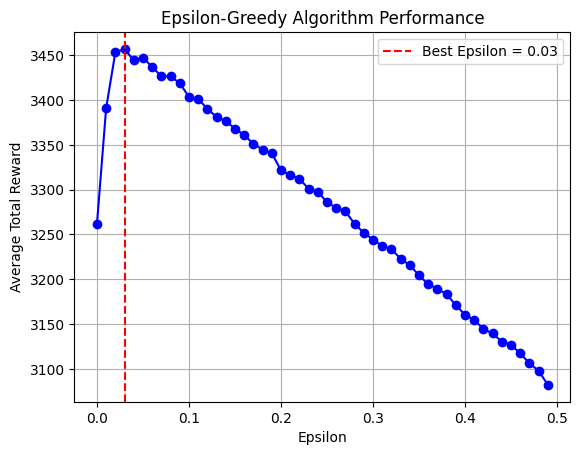
\includegraphics[width=\textwidth]{pics/greedy.png}
        \caption{\(\varepsilon\)-Greedy Results}
        \label{fig:epsilon_greedy}
    \end{subfigure}
    \hfill
    \begin{subfigure}[b]{0.45\textwidth}
        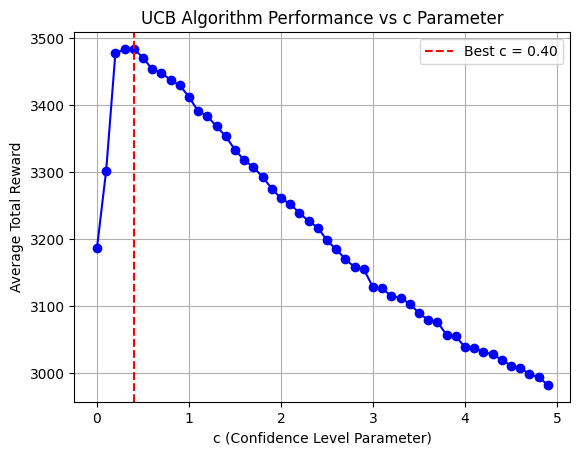
\includegraphics[width=\textwidth]{pics/ucb.png}
        \caption{UCB Results}
        \label{fig:ucb}
    \end{subfigure}
    \caption{Algorithm Performance Analysis}
    \label{fig:results}
\end{figure}

But even with the optimized parameters, the gap of the first two algorithms ($42.98$ and $16.10$ respectively) is still larger than \textbf{Thompson Sampling}, which has the smallest gap of $7.59$. Therefore, the \textbf{Thompson Sampling} algorithm is the best-performing algorithm in this scenario.


\subsubsection*{Parameter Impact Analysis}
\begin{enumerate}[1.]
\item \(\varepsilon\)-Greedy Algorithm

The \(\varepsilon\)-Greedy algorithm explores with probability \(\varepsilon\) and exploits with probability \(1 - \varepsilon\). The parameter \(\varepsilon\) controls the level of exploration versus exploitation.
\begin{itemize}
    \item \textbf{Low \(\varepsilon\) :}
    \begin{itemize}
        \item Pros: Prefer exploitation to exploration, leading to higher rewards when the current best action is optimal.
        \item Cons: Limited exploration may prevent discovery of better actions, especially in complex environments.
    \end{itemize}
    
    \item \textbf{High \(\varepsilon\) (e.g., \(\varepsilon = 0.5\)):}
    \begin{itemize}
        \item Pros: Increased exploration, potentially leading to the discovery of optimal actions.
        \item Cons: Excessive exploration dilutes the focus on known good actions, potentially lowering overall rewards.
    \end{itemize}
    
    \item \textbf{Optimal \(\varepsilon\):} Based on experiments, we find that \(\varepsilon = 0.03\) yields the highest average reward of 3457.02, indicating a good balance between exploration and exploitation. And when \(\varepsilon > 0.03\), the average reward decreases as the $\varepsilon$ (exploration) increases.
\end{itemize}

\item Upper Confidence Bound (UCB)

The UCB formula consists of two terms:

\begin{itemize}
    \item \textbf{Exploitation (\(\hat{\theta}(j)\)):} This term represents the current mean reward of action \(j\), which is used to exploit the known best action. The algorithm favors actions with a higher expected reward, leading to exploitation.
    
    \item \textbf{Exploration (\(c \cdot \sqrt{\frac{2 \ln(t)}{\text{count}(j)}}\)):} This term encourages exploration by adding a bonus to actions that have been chosen fewer times. The bonus is larger for actions that are less tested, which helps to balance exploration with the exploitation of known rewards. The parameter \(c\) controls the size of the exploration term. A higher \(c\) increases exploration, and a smaller \(c\) favors exploitation.
\end{itemize}
So the parameter \(c\) controls the trade-off between exploration and exploitation in the UCB algorithm, which is discussed as follows:
\begin{itemize}
    \item \textbf{Low \(c\):}
    \begin{itemize}
        \item Pros: Promotes exploitation as the confidence bounds become tighter.
        \item Cons: Reduced exploration can prevent the algorithm from discovering better actions.
    \end{itemize}
    
    \item \textbf{High \(c\):}
    \begin{itemize}
        \item Pros: Increases exploration by enlarging the confidence bounds, particularly for arms that have been pulled fewer times.
        \item Cons: Excessive exploration can reduce the focus on exploitation, potentially leading to suboptimal rewards.
    \end{itemize}
    
    \item \textbf{Optimal \(c\):} In our experiments, \(c = 0.40\) provides the best performance, yielding a maximum reward of 3483.90. And when \(c > 0.40\), the average reward decreases as the \(c\) (exploration) increases.
\end{itemize}

\item Thompson Sampling

The Thompson Sampling algorithm is a Bayesian method that uses prior and posterior beliefs to update the probability distribution for each action's reward. It assumes a Beta distribution as the prior for the reward probability of each arm, and updates the parameters \(\alpha_j\) and \(\beta_j\) based on the observed outcomes.

  \textbf{Prior Belief:}
    \begin{itemize}
        \item \(\alpha_j\) and \(\beta_j\) represent our prior belief about the reward distribution for action \(j\).
        \item For example, \(\alpha_j = 1\) and \(\beta_j = 1\) implies that we expect the reward probability for action \(j\) to be 50%, but we have low confidence in this belief (uniform distribution).
        \item A higher value of \(\alpha_j\) relative to \(\beta_j\) means that we believe the reward probability for action \(j\) is higher, whereas a lower value of \(\alpha_j\) relative to \(\beta_j\) suggests that we believe the reward probability is lower.
    \end{itemize}

  \textbf{Effect of \(\alpha_j\) and \(\beta_j\):}
    \begin{itemize}
        \item \(\alpha_j\) and \(\beta_j\) are updated after each trial, based on whether the reward for action \(j\) was successful or not.
        \item When \(\alpha_j\) is large and \(\beta_j\) is small (e.g., \(\alpha_j = 2000\), \(\beta_j = 8000\)), we have a strong belief that the probability of a reward is low (20\%), and the algorithm exploits this information.
        \item When both \(\alpha_j\) and \(\beta_j\) are small (e.g., \(\alpha_j = 1\), \(\beta_j = 1\)), there is high uncertainty about the reward distribution, encouraging more exploration of different actions.
    \end{itemize}

  \textbf{Balancing Exploration and Exploitation:}
    \begin{itemize}
        \item Thompson Sampling uses the Beta distribution to balance exploration and exploitation. Actions with higher posterior probability are more likely to be chosen, but there is still a chance of selecting suboptimal actions (exploration).
        \item The larger the parameters \(\alpha_j\) and \(\beta_j\), the more confident we are in the reward probability, and the less frequently our belief is updated. This reduces exploration and makes the algorithm focus more on exploitation.
    \end{itemize}
    
  \textbf{Effect of Prior Distribution:}
    \begin{itemize}
        \item If we set the prior \(\alpha_j\) and \(\beta_j\) values to be small, the agent explores more, as the uncertainty is high. This might lead to more exploration but fewer immediate rewards.
        \item If we set the prior to values close to the true expected reward (the oracle value), the algorithm will converge quickly to the best action, leading to better performance.
    \end{itemize}

\end{enumerate}

\newpage
\section{Part II: Bayesian Bandit Algorithms}

\bibliographystyle{plainnat}
\bibliography{references}  % references.bib file

\appendix

\end{document}